\setlength{\footskip}{8mm}

\chapter{Methodology}
\label{ch:methodology}

 In this chapter the methodology for implementing the ICPCR system is illustrated. Also the steps that would be followed are outlined.

\section{Research Methodology}
The following steps will be conducted also shown in Figure~\ref{fig:ResearchMethodology} :
\begin{enumerate}[label=Step \arabic*:]
	
	\item Data Preprocessing and Datawarehouse Development
	\begin{itemize}
		\item Data Collection
		\item Meta-data evaluation
		\item Data cleaning
		\item Datawarehouse design
		\item ETL process
	\end{itemize}
	\item Development and Evaluation of the Prediction Models
	\begin{itemize}
		\item Select three churn prediction models
		\item Models to be trained and tested with the data
		\item Model Evaluation
	\end{itemize}
	\item System Development \& Evaluation
	\begin{itemize}
		\item Build the ICPCR system as a web application.
		\item Integration of Web app with OLAP and prediction model.
		\item Develop the Dashboards to display KPI's.
		\item Test the system.
	\end{itemize}
\end{enumerate}

\begin{figure}[h!]
	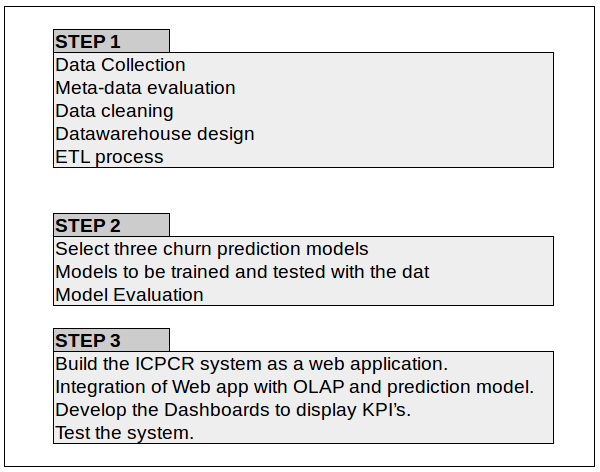
\includegraphics[scale = 0.5]{figures/ICPCR.png}
	\centering
	\caption{Research Methodology}
	\label{fig:ResearchMethodology}
\end{figure}
\newpage

\section{Data Preprocessing and Datawarehouse Development}

\subsection{Data preprocessing}

Data will be collected from available open source sites.
In this section a sequence of steps for data preparation are listed. In Figure \ref{fig:dataprerocessing} the process flow is shown.

\begin{enumerate}
	\item Study of meta-data of the dataset. This study reveals the important attributes to be used for prediction.
	\item Cleaning of un-usable data, either by replacing with suitable or by entirely removing it. Un-usable data is the one that may be invalid like null or special characters in numeric fields etc.
	\item Extract the data and load into the database. This helps in querying the data faster with Structured Query Language.
\end{enumerate}

\begin{figure}[h]
	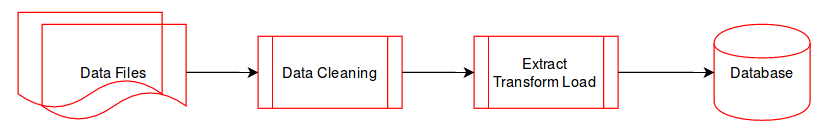
\includegraphics[scale = 0.5]{figures/dataloadprocess.png}
	\centering
	\caption{Data preprocessing}
	\label{fig:dataprerocessing}
\end{figure}


\subsection{Datawarehouse development}
Following steps will be followed for design of data warehouse:

The attributes generated from above step are summarized. This summary is used to design the OLAP cube. The OLAP will be used in generating reports and KPI's for the dashboard generation. The OLAP will be designed with the star schema. Figure~\ref{fig:olapstarschema} shows a typical implementation of the star schema \shortcite{olapstarschema}. A similar structure will be implemented for the study after the dimensions of the data are finalized.

Like for example the count of all the people between the age of 22 to 24 using prepaid service for the year 2013 could be one data whereas the count for 2014 would be another.

 \begin{figure}[h]
 	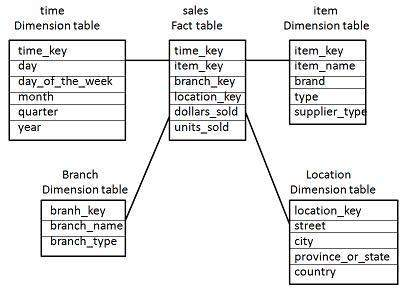
\includegraphics[scale = 0.7]{figures/olap_start_schema.jpg}
 	\centering
 	\caption{OLAP Star Schema}
 	\label{fig:olapstarschema}
 \end{figure}


After the Datawarehouse is designed, the tables have to be loaded with data. Thus the next step of ETL is done.
Extract Transform and Load processing (ETL) This is a necessary step that would be required to properly extract data from the data file, transform the data types in order that they may be suitable for the database and finally loading to database.
 
\newpage
\section{Development and Evaluation of the Prediction Models}
\subsection{Model Design}
In this section, the models are selected for churn prediction. Tentatively it is decided to select Decision tree, Support Sector Machine and ANN. The models will be trained with a training set and then the performance will be evaluated with the testing set. The proposal is to select either the machine learning library of MLib under Apache or Scikit of Python or libraries under R. It will largely depend on the availability of the models in the libraries. In case a model is not available it will be sourced from another library. Also in addition it is proposed that a boosting algorithm like Adaboost would be used to measure change in prediction performance.

\subsection{Model Evaluations}
In order to judge the better performing model or rather the accuracy of predictability by the classification techniques, it is but necessary to perform an evaluation. The evaluations that are commonly performed by academicians are the k-Fold Cross Validation, Sensitivity \& Specificity measurements \shortcite{lariviere2005predicting}.\\
\begin{itemize}
	\item K-Fold Cross Validation : It is proposed to per form this process to make the classification model more accurate. From previous literature it is learned that k = 100 is highly appropriate.
	\item Plotting of confusion matrix, as followed by other academicians and then deriving the Sensitivity, Specificity, Precision, Recall and F-score are the proposed evaluation techniques
\end{itemize}

\newpage
\section{System Development \& Evaluation}
In this section the architecture of the ICPCR system is proposed. The application, shown in Figure \ref{fig:system-design-churn-prediction}, would be developed in a 3-tire format i.e, Database Layer, Application Layer, and Presentation Layer. The system is designed in two modes. One is the learning phase mode and the other is the Prediction phase mode. In the learning phase the system is fed data and the inference engine learns the trend. Testing and benchmarking along with weighting.
\begin{figure}[h]
	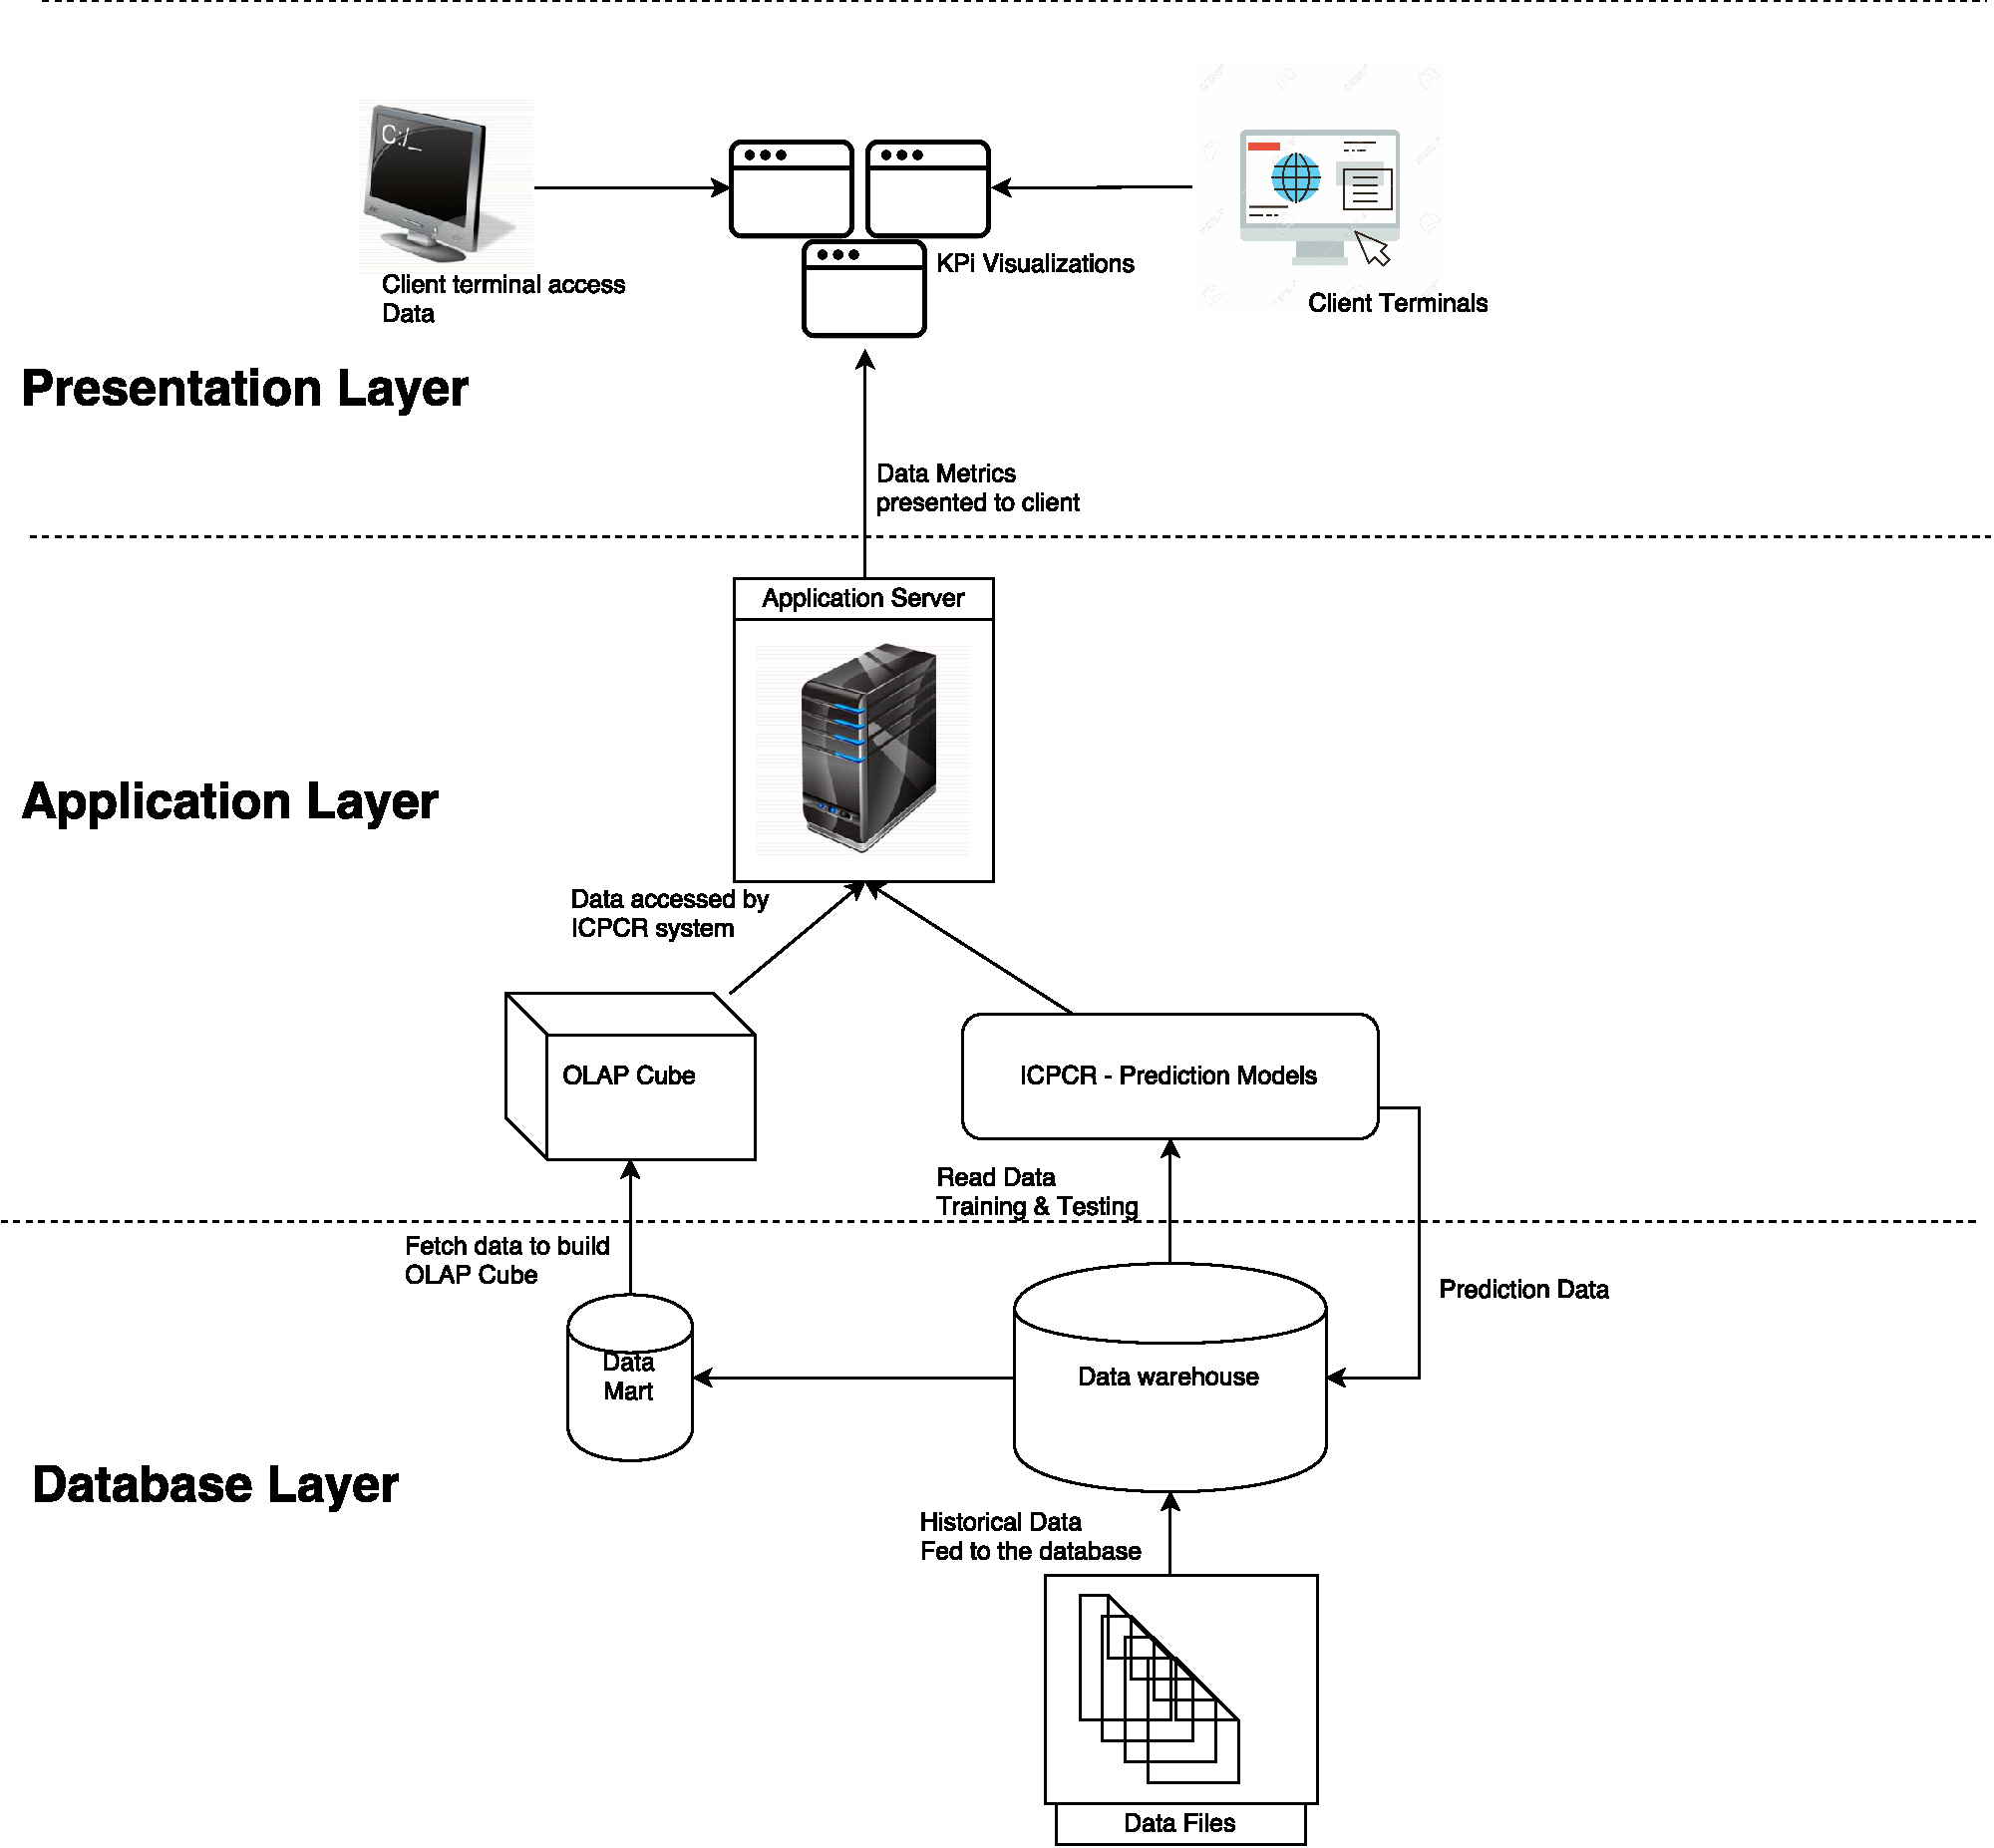
\includegraphics[width=\textwidth]{figures/ICPCR_pic1SystemDesign}
	\centering
	\caption{The Intelligent Churn Prediction Architecture}
	\label{fig:system-design-churn-prediction}
\end{figure}



\subsection{Presentation Layer}
In this thesis, the presentation layer is the section of the system which is accessible to the user or client. This is used to view the key values obtained from the OLAP and the mining results. There would be a display of metrics of the data.
\begin{enumerate}
	\item It is proposed to deploy a suitable application to display a dashboard of KPI's.
	\item The display of KPI's will be in graphs and charts format. The KPI's are taken from the OLAP cube.
\end{enumerate}


\subsection{Application Layer}
This layer would be comprised of three parts.
\begin{enumerate}
	\item Application server : This consists of the set of logic codes which will fetch the appropriate data for display in the front end. It may fetch the data directly from the tables or from the OLAP Cube, as is requested from the user.
	\item Prediction model : This part is comprised of the predictive model to predict the outcome of data presented to it in the database. The model will go through a phase of training, testing, and prediction of churn value for new data. Also it is proposed that Prediction model be able to identify the variables which could be addressed for retaining the customer.
	\item OLAP : This is the MOLAP implementation for building the Key metrics from the data. This part of the system would be responsible for the dashboard metrics display to the user.
\end{enumerate}


\subsection{Database Layer}
This layer will be comprised of the data-warehouse tables. The OLAP calculation and the Model predictions will be updated whensoever a set of ne data is identified. The Olap cube feed tables will also be present here. A Star schema will be implemented for fetching of data for the various dimensions of the OLAP.

\subsection{System Evaluation}
The thesis proposes a system evaluation process to audit the performance. A set of test from latency in display and run will be calculated and improved before the process of deployment. This would ensure that system does not behave erratically under normal situations.

\newpage
\begin{landscape}
\section{Timeline}
 The forecast of the tasks to be carried out in this thesis are shown below in a Gantt chart Figures~\ref{fig:time1}.
 \\
  \begin{figure}[H]
  	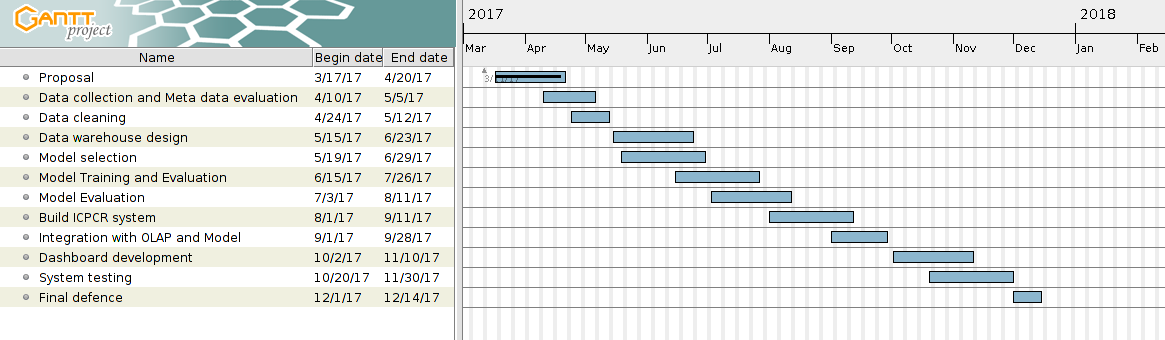
\includegraphics[width=25cm, height=10cm]{figures/churngantt3.png}
  	\centering
  	\caption{Gantt chart tasks}
  	\label{fig:time1}
  \end{figure}
\end{landscape}
% \begin{landscape}


%\begin{figure}[h]
%    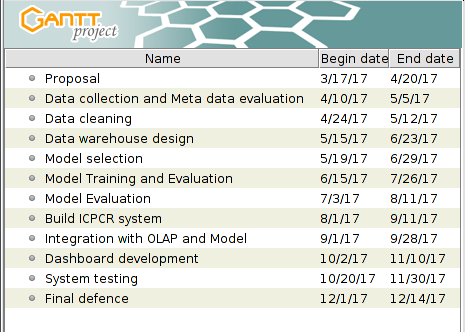
\includegraphics[scale=0.75]{figures/churngantt1.png}
% 	\caption{Gantt chart task}
% 	\label{fig:time2}
% \end{figure}

% \begin{figure}[h]
%	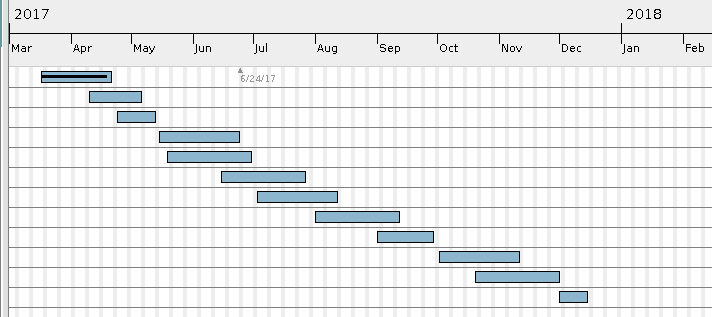
\includegraphics[scale=0.75]{figures/churngantt2.png}
% 	\caption{Gantt chart durations}
% 	\label{fig:time1}
% \end{figure}

%\newpage


%\end{landscape}

\FloatBarrier
